\chapter{Sistema actual: plataforma FAdA}
\label{chap:sistema_original}

\textcolor{red}{En este capitulo describiremos el funcionamiento del sistema actual, aquel que queremos dividir en microservicios. Repasaremos su implementación, su estructura actual y qué queremos lograr. Exploraremos sus componentes y describiremos nuestros objetivos para dividirlo.}

\begin{wrapfigure}{r}{0.3\linewidth}
  \centering
  
\includegraphics[scale=0.45]{cap_sistema_original/images/fada-logo}
\end{wrapfigure}

La plataforma FAdA\footnote{Página oficial: \url{http://fada.tatami.webs.upv.es/}} está enfocada en el desarrollo de sistemas autoadaptativos. Es un desarrollo del grupo PROS/Tatami\footnote{Página oficial: \url{http://www.pros.webs.upv.es/}} del instituto VRAIN/UPV\footnote{Página oficial: \url{https://vrain.upv.es/}}. Está compuesta por una serie de herramientas y guías metodológicas. Entre ellas encontramos extensiones de modelado para el IDE Eclipse, generadores de código y diversas implementaciones de bucles de control genéricos.

\section{Desarrollo de servicios \foreign{english}{Adaptive Ready}}

Comenzaremos describiendo la extensión para el IDE Eclipse. Tomando una aproximación de \textbf{desarrollo dirigido por modelos} (o \foreign{english}{model driven development}, MDD), esta herramienta permite diseñar soluciones autoadaptativas. Las soluciones están compuestas por especificaciones de servicios \textbf{\foreign{english}{adaptive ready}} (ARS). \cite{fonsServiciosAdaptivereadyPara2021} Se trata de servicios que ofrecen una serie de interfaces o \foreign{english}{touchpoints} que permiten manipularlos desde un bucle de control externo. En la figura \ref{fig:adaptive-ready-services} mostramos un esquema del servicio y de cómo el bucle orquesta la solución.

A partir de los modelos, podemos generar código para los servicios. La plataforma ofrece una serie de generadores para el lenguaje Java. Basándose en la especificación, generarán todo el código de infraestructura para dar soporte a estas interfaces de adaptación. Para integrarlas con nuestro sistema, deberemos implementar la lógica asociada a los comandos e importar el módulo en nuestra solución. Dependiendo del tipo de despliegue por el que optemos, pueden generar microservicios, módulos OSGi\footnote{Página oficial: \url{https://www.osgi.org}.}, entre otros.

Para operar estas soluciones, la plataforma ofrece distintas implementaciones de bucles de control. Dependen también del modelo de despliegue que elijamos. Disponemos de soluciones para gestionar microservicios sobre la plataforma Kubernetes\cite{fonsServiciosAdaptivereadyPara2021}, otros que permiten operar componentes OSGi\footnote{Página oficial: \url{https://www.osgi.org}.}, etc. Para este trabajo nos centraremos en una versión reducida del bucle de control para microservicios: MAPE-K \foreign{english}{Lite}.

\begin{figure}[htb]
  \centering
  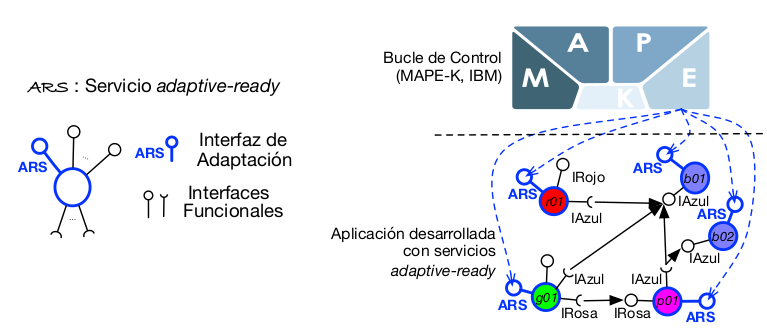
\includegraphics[scale=0.4]{cap_sistema_original/images/adaptive-ready-services}
  \caption[Servicio adaptive-ready y Bucle MAPE-K sobre arquitectura de mi-
  croservicios adaptive-ready.]{Servicio adaptive-ready (izquierda) y Bucle MAPE-K sobre arquitectura de microservicios adaptive-ready (derecha). Obtenida de \cite{fonsServiciosAdaptivereadyPara2021}.}
  \label{fig:adaptive-ready-services}
\end{figure}


\section{Bucle de control MAPE-K \foreign{english}{Lite}}

El bucle de control MAPE-K \foreign{english}{Lite} de FAdA nos permite gestionar soluciones autoadaptativas basadas en microservicios. Es una versión reducida del bucle presentado en \cite{fonsEspecificacionSistemasAutoadaptativos2021}. Sigue la arquitectura MAPE-K descrita en la sección \ref{sec:bucles-mapek}. En su implementación actual, se despliega como un servicio monolítico. Todos sus componentes, tanto del bucle como los del recurso manejado (monitores, reglas..), se ejecutan dentro del mismo proceso.

El bucle de control es genérico. No está acoplado a un dominio o solución concreta. Además pueden hacer uso de él varios sistemas. El proceso acepta como entradas las mediciones de las sondas y emite comandos dirigidos a los efectores del recurso manejado. En nuestro caso, los \foreign{english}{touchpoints} de los servicios adaptive ready. En la figura \ref{fig:bucle-mapek3} mostramos un modelo que detalla el flujo de control e información dentro de sus etapas.

\begin{figure}[htb]
  \centering
  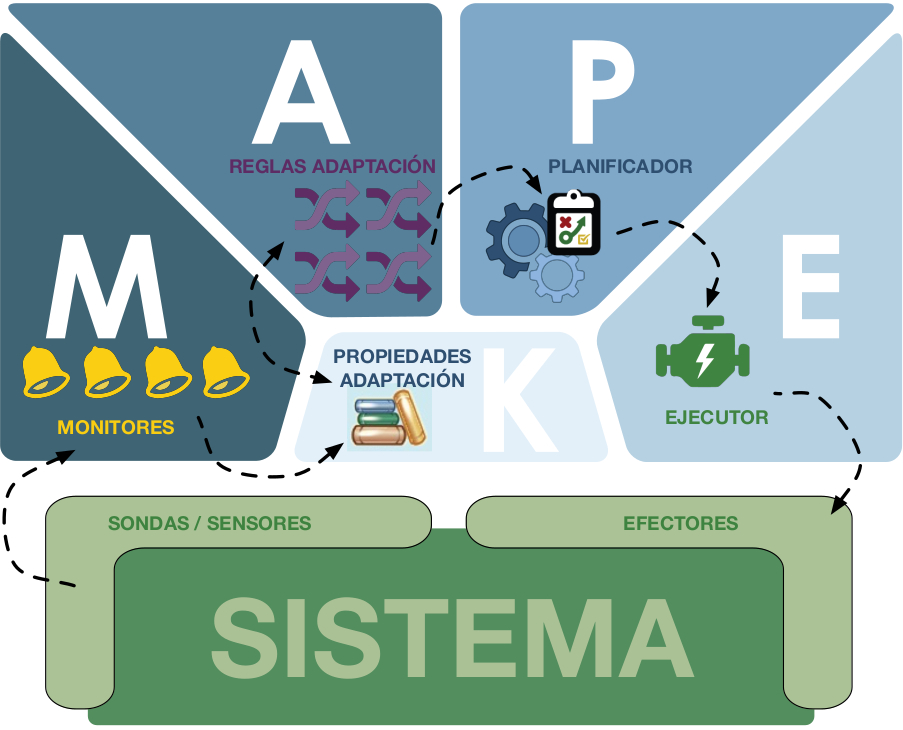
\includegraphics[scale=1.1]{cap_introduccion/images/bucle-mape-k}
  \caption[Arquitectura de un Bucle MAPE-K. El flujo de información y de control entre las etapas del bucle están representados con flechas.]{Arquitectura de un Bucle MAPE-K. El flujo de información y de control entre las etapas del bucle están representados con flechas. Obtenida de \cite{fonsEspecificacionSistemasAutoadaptativos2021}}
  \label{fig:bucle-mapek3}
\end{figure}

\subsection{Estructura del bucle}

En la sección \ref{sec:estructura-mape-k} ya describimos la estructura de un bucle MAPE-K típico. Como vemos ver en la figura \ref{fig:bucle-mapek3}, este no difiere mucho en su implementación. Utiliza los mismos componentes: sondas, monitores, módulo de análisis, planificador, ejecutor y efectores. Pero sí que hay facetas en las que queremos hacer hincapié: el uso de reglas de adaptación para implementar la etapa de análisis; y el uso de los operadores arquitectónicos para microservicios.

\subsubsection{Operadores arquitectónicos}

Las adaptaciones que realiza un sistema autoadaptativo están compuestas por acciones. Estas acciones modifican la configuración o la arquitectura del sistema en tiempo de ejecución. Dependiendo del estilo arquitectónico, tendremos disponibles acciones de distintos tipos. Por lo general suelen ser muy similares: añadir o eliminar componentes, modificar las conexiones entre ellos o cambiar parámetros de configuración. Estas se describen con \textbf{operadores arquitectónicos}. \cite{garlanIncreasingSystemDependability2003}

El bucle de control que nos ocupa es específico para gestionar soluciones basadas en microservicios. Por tanto, ofrecerá los operadores arquitectónicos correspondientes a este estilo. En \cite{fonsEspecificacionSistemasAutoadaptativos2021} podemos ver las cinco tipos que soporta:

\begin{itemize}
  \item \textbf{Desplegar servicios} (\textbf{\foreign{english}{deploy}}): Añadimos una nueva instancia de un servicio.

  \item \textbf{Eliminar servicios} (\textbf{\foreign{english}{undeploy}}): Eliminamos una instancia de un servicio.

  \item \textbf{Enlazar servicios} (\textbf{\foreign{english}{bind}}): Añadimos una conexión entre dos servicios. A partir de entonces podrán comunicarse.

  \item \textbf{Desenlazar servicios} (\textbf{\foreign{english}{unbind}}): Eliminamos una conexión existente entre dos servicios. Ya no podrán comunicarse.

  \item \textbf{Cambiar configuración} (\textbf{\foreign{english}{set parameter}}): Modificamos un parámetro de configuración de un servicio.
\end{itemize}

En la figura \ref{fig:adaptaciones-microservicios} mostramos un ejemplo de los efectos de estas acciones en la arquitectura del sistema.

\begin{figure}[htb]
  \centering
  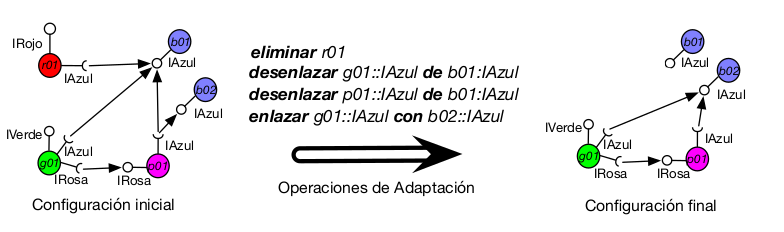
\includegraphics[scale=1.8]{cap_sistema_original/images/adaptaciones}
  \caption[Ejemplo de adaptaciones en un sistema basado en microservicios.]{Ejemplo de adaptaciones en un sistema basado en microservicios. Imagen original obtenida de \cite{fonsServiciosAdaptivereadyPara2021}}
  \label{fig:adaptaciones-microservicios}
\end{figure}


\subsubsection{Módulo de análisis y reglas de adaptación}

\textcolor{red}{Añadir ejemplo de regla de adaptación del climatizador}.

Para implementarlo, una posible aproximación es mediante \textbf{reglas de adaptación}. Estas pueden dividirse en dos partes: la condición y la acción. La condición se define a partir de las propiedades de adaptación y evalúa si es necesario ejecutar la acción correctiva.

La acción de la regla describe una \textbf{propuesta de cambio} en la configuración del sistema. Estas se formulan en base a \textbf{operadores arquitectónicos}. \cite{garlanIncreasingSystemDependability2003} Dependiendo del estilo arquitectónico de nuestro sistema, tendremos disponibles una serie de operaciones para alterar su arquitectura.

Por ejemplo, nuestro recurso manejado podría estar implementado como microservicios. En este caso, los operadores podrían consistir en desplegar o eliminar servicios, establecer conexiones entre los servicios, eliminarlas, o cambiar las propiedades de configuración del servicio. \cite{fonsServiciosAdaptivereadyPara2021}

Las reglas se suscriben a cambios de las propiedades de las que dependen. Cuando ocurra alguno, se evalúa su condición. Si esta se cumple, se ejecuta la acción asociada. En caso contrario, no hará nada.

Respecto al servicio web, definiremos reglas tomando el valor del número de peticiones por segundo. Podemos definirlas con umbrales para este valor: si es muy alto, la regla solicita el despliegue de una nueva instancia. Cuando la carga baje, y si el servicio está replicado, podremos eliminarlas.


Los servicios adaptive ready son agnósticos a la la lógica de las adaptaciones. Simplemente implementan su funcionalidad y los contratos de adaptación. Desde el bucle de control reciben los comandos de adaptación a través de sus efectores.
